\documentclass{standalone}
\usepackage{tikz, xcolor}
\usetikzlibrary{shapes,arrows}

\begin{document}

\begin{tikzpicture}[thick, scale=2.0]
\tikzstyle{vertexr}=[rectangle, draw=blue, thick, minimum size=14pt, inner sep=2pt]
\tikzstyle{vertexc}=[circle, draw=blue, thick, inner sep=2pt]
\tikzstyle{drawstyle}=[thick, ->]

\node[vertexr] (G0x0) at (0,0) {bool gx};
\node[vertexr] (G1x0) at (1,0) {bool gy};
\node[vertexr] (G2x0) at (2,0) {void Func esperanza};
\node[vertexr] (G2x1) at (2,-1) {bool px};
\node[vertexr] (G3x1) at (3,-1) {bool py};
\draw[drawstyle] (G2x1) -- (G3x1);
\draw[drawstyle] (G2x0) -- (G2x1);
\node[vertexr] (G4x1) at (4,-1) {Compound};
\node[vertexr] (G4x2) at (4,-2) {bool x};
\node[vertexr] (G5x2) at (5,-2) {bool y};
\node[vertexr] (G6x2) at (6,-2) {bool sx};
\node[vertexr] (G7x2) at (7,-2) {bool sy};
\draw[drawstyle] (G6x2) -- (G7x2);
\draw[drawstyle] (G5x2) -- (G6x2);
\draw[drawstyle] (G4x2) -- (G5x2);
\draw[drawstyle] (G4x1) -- (G4x2);
\node[vertexr] (G8x2) at (8,-2) {=};
\node[vertexr] (G8x3) at (8,-3) {gx};
\draw[drawstyle] (G8x2) -- (G8x3);
\node[vertexr] (G9x3) at (9,-3) {true};
\draw[drawstyle] (G8x2) -- (G9x3);
\node[vertexr] (G10x2) at (10,-2) {Call outputb};
\node[vertexr] (G10x3) at (10,-3) {gx};
\draw[drawstyle] (G10x2) -- (G10x3);
\node[vertexr] (G11x2) at (11,-2) {=};
\node[vertexr] (G11x3) at (11,-3) {gy};
\node[vertexr] (G11x4) at (11,-4) {9};
\draw[drawstyle] (G11x3) -- (G11x4);
\draw[drawstyle] (G11x2) -- (G11x3);
\node[vertexr] (G12x3) at (12,-3) {true};
\draw[drawstyle] (G11x2) -- (G12x3);
\node[vertexr] (G13x2) at (13,-2) {Call outputb};
\node[vertexr] (G13x3) at (13,-3) {gy};
\node[vertexr] (G13x4) at (13,-4) {9};
\draw[drawstyle] (G13x3) -- (G13x4);
\draw[drawstyle] (G13x2) -- (G13x3);
\node[vertexr] (G14x2) at (14,-2) {=};
\node[vertexr] (G14x3) at (14,-3) {x};
\draw[drawstyle] (G14x2) -- (G14x3);
\node[vertexr] (G15x3) at (15,-3) {true};
\draw[drawstyle] (G14x2) -- (G15x3);
\node[vertexr] (G16x2) at (16,-2) {Call outputb};
\node[vertexr] (G16x3) at (16,-3) {x};
\draw[drawstyle] (G16x2) -- (G16x3);
\node[vertexr] (G17x2) at (17,-2) {=};
\node[vertexr] (G17x3) at (17,-3) {y};
\node[vertexr] (G17x4) at (17,-4) {9};
\draw[drawstyle] (G17x3) -- (G17x4);
\draw[drawstyle] (G17x2) -- (G17x3);
\node[vertexr] (G18x3) at (18,-3) {true};
\draw[drawstyle] (G17x2) -- (G18x3);
\node[vertexr] (G19x2) at (19,-2) {Call outputb};
\node[vertexr] (G19x3) at (19,-3) {y};
\node[vertexr] (G19x4) at (19,-4) {9};
\draw[drawstyle] (G19x3) -- (G19x4);
\draw[drawstyle] (G19x2) -- (G19x3);
\node[vertexr] (G20x2) at (20,-2) {Call outnl};
\node[vertexr] (G21x2) at (21,-2) {=};
\node[vertexr] (G21x3) at (21,-3) {px};
\draw[drawstyle] (G21x2) -- (G21x3);
\node[vertexr] (G22x3) at (22,-3) {true};
\draw[drawstyle] (G21x2) -- (G22x3);
\node[vertexr] (G23x2) at (23,-2) {Call outputb};
\node[vertexr] (G23x3) at (23,-3) {px};
\draw[drawstyle] (G23x2) -- (G23x3);
\node[vertexr] (G24x2) at (24,-2) {=};
\node[vertexr] (G24x3) at (24,-3) {py};
\node[vertexr] (G24x4) at (24,-4) {9};
\draw[drawstyle] (G24x3) -- (G24x4);
\draw[drawstyle] (G24x2) -- (G24x3);
\node[vertexr] (G25x3) at (25,-3) {true};
\draw[drawstyle] (G24x2) -- (G25x3);
\node[vertexr] (G26x2) at (26,-2) {Call outputb};
\node[vertexr] (G26x3) at (26,-3) {py};
\node[vertexr] (G26x4) at (26,-4) {9};
\draw[drawstyle] (G26x3) -- (G26x4);
\draw[drawstyle] (G26x2) -- (G26x3);
\node[vertexr] (G27x2) at (27,-2) {=};
\node[vertexr] (G27x3) at (27,-3) {sx};
\draw[drawstyle] (G27x2) -- (G27x3);
\node[vertexr] (G28x3) at (28,-3) {true};
\draw[drawstyle] (G27x2) -- (G28x3);
\node[vertexr] (G29x2) at (29,-2) {Call outputb};
\node[vertexr] (G29x3) at (29,-3) {sx};
\draw[drawstyle] (G29x2) -- (G29x3);
\node[vertexr] (G30x2) at (30,-2) {=};
\node[vertexr] (G30x3) at (30,-3) {sy};
\node[vertexr] (G30x4) at (30,-4) {9};
\draw[drawstyle] (G30x3) -- (G30x4);
\draw[drawstyle] (G30x2) -- (G30x3);
\node[vertexr] (G31x3) at (31,-3) {true};
\draw[drawstyle] (G30x2) -- (G31x3);
\node[vertexr] (G32x2) at (32,-2) {Call outputb};
\node[vertexr] (G32x3) at (32,-3) {sy};
\node[vertexr] (G32x4) at (32,-4) {9};
\draw[drawstyle] (G32x3) -- (G32x4);
\draw[drawstyle] (G32x2) -- (G32x3);
\node[vertexr] (G33x2) at (33,-2) {Call outnl};
\draw[drawstyle] (G32x2) -- (G33x2);
\draw[drawstyle] (G30x2) -- (G32x2);
\draw[drawstyle] (G29x2) -- (G30x2);
\draw[drawstyle] (G27x2) -- (G29x2);
\draw[drawstyle] (G26x2) -- (G27x2);
\draw[drawstyle] (G24x2) -- (G26x2);
\draw[drawstyle] (G23x2) -- (G24x2);
\draw[drawstyle] (G21x2) -- (G23x2);
\draw[drawstyle] (G20x2) -- (G21x2);
\draw[drawstyle] (G19x2) -- (G20x2);
\draw[drawstyle] (G17x2) -- (G19x2);
\draw[drawstyle] (G16x2) -- (G17x2);
\draw[drawstyle] (G14x2) -- (G16x2);
\draw[drawstyle] (G13x2) -- (G14x2);
\draw[drawstyle] (G11x2) -- (G13x2);
\draw[drawstyle] (G10x2) -- (G11x2);
\draw[drawstyle] (G8x2) -- (G10x2);
\draw[drawstyle] (G4x1) -- (G8x2);
\draw[drawstyle] (G2x0) -- (G4x1);
\node[vertexr] (G34x0) at (34,0) {void Func main};
\node[vertexc] (G34x1) at (34,-1) {.};
\draw[drawstyle] (G34x0) -- (G34x1);
\node[vertexr] (G35x1) at (35,-1) {Compound};
\node[vertexr] (G35x2) at (35,-2) {bool zx};
\node[vertexr] (G36x2) at (36,-2) {bool zy};
\draw[drawstyle] (G35x2) -- (G36x2);
\draw[drawstyle] (G35x1) -- (G35x2);
\node[vertexr] (G37x2) at (37,-2) {Call esperanza};
\node[vertexr] (G37x3) at (37,-3) {zx};
\node[vertexr] (G38x3) at (38,-3) {zy};
\draw[drawstyle] (G37x3) -- (G38x3);
\draw[drawstyle] (G37x2) -- (G37x3);
\draw[drawstyle] (G35x1) -- (G37x2);
\draw[drawstyle] (G34x0) -- (G35x1);
\draw[drawstyle] (G2x0) -- (G34x0);
\draw[drawstyle] (G1x0) -- (G2x0);
\draw[drawstyle] (G0x0) -- (G1x0);
\end{tikzpicture}
\end{document}
Number of warnings: 0
Number of errors: 0
